\documentclass[a4paper,parskip,11pt, DIV12]{scrreprt}

\usepackage[ngerman]{babel} % FÌr Deutsch [english] zu [ngerman] Àndern. 
\usepackage[utf8]{inputenc}
\usepackage[T1]{fontenc}
\usepackage{blindtext}
\usepackage{graphicx}
\usepackage{subfigure}
%\renewcommand{\familydefault}{\sfdefault}
\usepackage{fancyhdr}
\usepackage{amsmath}
\usepackage{mdwlist} %Benötigt fÌr AbstÀnde in AufzÀhlungen zu löschen
\usepackage{here}
\usepackage{calc}
\usepackage{hhline}
\usepackage{marginnote}
\usepackage{chngcntr}
\usepackage{helvet}
\usepackage{tabularx}
\usepackage{titlesec} % TextÃŒberschriften anpassen

% \titleformat{Überschriftenklasse}[Absatzformatierung]{Textformatierung} {Nummerierung}{Abstand zwischen Nummerierung und Überschriftentext}{Code vor der Überschrift}[Code nach der Überschrift]

% \titlespacing{Überschriftenklasse}{Linker Einzug}{Platz oberhalb}{Platz unterhalb}[rechter Einzug]

\titleformat{\chapter}{\LARGE\bfseries}{\thechapter\quad}{0pt}{}
\titleformat{\section}{\Large\bfseries}{\thesection\quad}{0pt}{}
\titleformat{\subsection}{\large\bfseries}{\thesubsection\quad}{0pt}{}
\titleformat{\subsubsection}{\normalsize\bfseries}{\thesubsubsection\quad}{0pt}{}

\titlespacing{\chapter}{0pt}{-2em}{6pt}
\titlespacing{\section}{0pt}{6pt}{-0.2em}
\titlespacing{\subsection}{0pt}{5pt}{-0.4em}
\titlespacing{\subsubsection}{0pt}{-0.3em}{-1em}

%\usepackage[singlespacing]{setspace}
%\usepackage[onehalfspacing]{setspace}

\usepackage[
			%includemp,				%marginalien in Textkörper einbeziehen
			%includeall,
			%showframe,				%zeigt rahmen zum debuggen		
			marginparwidth=25mm, 	%breite der marginalien
			marginparsep=5mm,		%abstand marginalien - text
			reversemarginpar,		%marginalien links statt rechts
			%left=50mm,				%abstand von Seitenraendern
%			top=25mm,				%
%			bottom=50mm,
			]{geometry}		

%Bibliographie- Einstellungen
\usepackage[babel,german=quotes]{csquotes}
\usepackage[
   backend=bibtex8, 
   natbib=true,
    style=numeric,
    sorting=none
]{biblatex}
\bibliography{Quelle}
%Fertig Bibliographie- Einstellungen

\usepackage{hyperref}

\newcommand{\footnoteremember}[2]{
  \footnote{#2}
  \newcounter{#1}
  \setcounter{#1}{\value{footnote}}
}
\newcommand{\footnoterecall}[1]{%
  \footnotemark[\value{#1}]
}

\begin{document}
\selectlanguage{ngerman}
\begin{titlepage}
\begin{figure}[h]
\hfill
\subfigure{
\includegraphics[scale=0.04]{uzh}}
\end{figure}
\vspace{1 cm}
\textbf{\begin{huge}Praktikumsbericht Festkörperphysik
\end{huge}}\\
\noindent\rule{\textwidth}{1.1 pt} \\

\begin{Large}\textbf{Widerstandsmessung an einem Halbleiter}
\end{Large}\\ 
\normalsize 
\par
\begingroup
\leftskip 0 cm
\rightskip\leftskip
\textbf{Modul:}\\ PHY210 \\ \\
\textbf{Assistent:}\\ Kay Waltar\\ \\
\textbf{Studenten:}\\ Manuel Sommerhalder, Fabian Stäger, Nora Salgo\\ \\
\textbf{Datum des Versuchs:}\\ 16.06.2017 \\ \\
\par
\endgroup
\clearpage



\end{titlepage}


%Start Layout
\pagestyle{fancy}
\fancyhead{} 
\fancyhead[R]{\small \leftmark}
\fancyhead[C]{\textbf{Halbleiter} } 
\fancyhead[L]{
\includegraphics[height=2\baselineskip]{uzh}}

\fancyfoot{}
\fancyfoot[R]{\small \thepage}
\fancyfoot[L]{}
\fancyfoot[C]{}
\renewcommand{\footrulewidth}{0.4pt} 

\addtolength{\headheight}{2\baselineskip}
\addtolength{\headheight}{0.6pt}


\renewcommand{\headrulewidth}{0.6pt}
\renewcommand{\footrulewidth}{0.4pt}
\fancypagestyle{plain}{				% plain redefinieren, damit wirklich alle seiten im gleichen stil sind (ausser titlepage)
\pagestyle{fancy}}

\renewcommand{\chaptermark}[1]{ \markboth{#1}{} } %Das aktuelle Kapitel soll nicht Gross geschriben und Nummeriertwerden

\counterwithout{figure}{chapter}
\counterwithout{table}{chapter}
%Ende Layout

\tableofcontents

\chapter{Physikalischer Hintergrund}
\label{ch:Physik}

Für das Experiment wird der Widerstand einer Siliziumprobe bei verschiedenen Temperaturen gemessen. Bei reinem Silizium handelt es sich um einen intrinsischen Halbleiter. Somit besteht die Ladungsträgerdichte zu gleichen Teilen aus einem Elektronenanteil $n$ und einem Lochanteil $p$.
Die elektrische Leitfähigkeit eines Halbleiters ist gegeben durch die Formel\footnoteremember{kittel}{Introduction to solid state physics / Charles Kittel.—8th ed.}
\begin{equation}
\label{eq:sigma}
\sigma = ne\mu_e + pe\mu_h ,
\end{equation}
wobei $\mu_e$ und $\mu_h$ jeweils die Mobilität der Elektronen- bzw. Loch-Beiträge ist. Diese ist leicht temperaturabhängig. Die Elektronenladungsdichte $n$ errechnet sich aus der Formel\footnoterecall{kittel}
\begin{equation}
n = \int_{E_c}^{\infty} D_e(E) f_e(E) dE 
\end{equation}
mit der Zustandsdichte\footnoterecall{kittel}
\begin{equation}
D_e(E) = \frac{1}{2 \pi^2} \left(\frac{2 m_e}{\hbar^2}\right)^{3/2} (E - E_c)^{1/2}
\end{equation}
($m_e$ ist die effektive Masse, $\hbar$ die reduzierte Planck-Konstante und $E_c$ die niedrigste Energie des Leitungsbandes) und der Fermi-Dirac-Statistik\footnoterecall{kittel}
\begin{equation}
f(E,T) = \frac{1}{\exp \left(\frac{\mu - E}{k_B T}\right) + 1}
\end{equation}
($\mu$ ist hier das chemische Potential), was sich mit der Näherung $\mu - E >> k_B T$ integrieren lässt zu\footnoterecall{kittel}
\begin{equation}
n = 2 \left(\frac{m_e k_B T}{2 \pi \hbar^2}\right)^{3/2} \exp \left(\frac{\mu - E_c}{k_B T}\right).
\end{equation}
Ganz analog errechnet sich die Lochdichte mit derselben Näherung zu\footnoterecall{kittel}
\begin{equation}
p = 2 \left(\frac{m_h k_B T}{2 \pi \hbar^2}\right)^{3/2} \exp \left(\frac{E_v - \mu}{k_B T}\right)
\end{equation}
($E_v$ ist die höchste Energie des Valenzbandes). Das Produkt von $n$ und $p$ ist somit nur von der Temperatur abhängig:
\begin{equation}
np = 4 \left(\frac{k_B T}{2 \pi \hbar^2}\right)^{3} (m_e m_h)^{3/2} \exp \left(\frac{-E_g}{k_B T}\right)
\end{equation}
Dabei ist $E_g = E_c – E_v$ die Energiebandlücke. Da die beiden Ladungsdichten im intrinsischen Fall gleich gross sind, lassen sie sich durch Folgende Formel in Abhängigkeit der Bandlücke und der Temperatur beschreiben:
\begin{equation}
n = p = 2 \left(\frac{k_B T}{2 \pi \hbar^2}\right)^{3/2} (m_e m_h)^{3/4} \exp \left(\frac{-E_g}{2 k_B T}\right)
\end{equation}
Der spezifische Widerstand ist somit nach einsetzen in Formel \ref{eq:sigma}
\begin{equation}
\rho = \frac{1}{\sigma} = \frac{1}{2 (\mu_e + \mu_h)e} \left(\frac{k_B T}{2 \pi \hbar^2}\right)^{-3/2} (m_e m_h)^{-3/4} \exp \left(\frac{E_g}{2 k_B T}\right)
\end{equation}
Da der elektrische Widerstand mit einem geometrischen Faktor direkt proportional zum spezifischen Widerstand ist, wird dieser somit
\begin{equation}
\label{eq:Endloesung}
R = A(T) T^{-3/2} \exp \left(\frac{E_g}{2 k_B T}\right)
\end{equation}
mit $A(T)$ als leicht temperaturabhängigem Proportionalitätsfaktor. 

\chapter{Experimenteller Aufbau}
Die Silizium-Probe ist auf einem isolierenden Probeträger aus Keramikmaterial angebracht. An diesem zylinderförmigen Träger sind die Kontakte für die Vierpunktmessung des Widerstandes angebracht, sowie ein Thermoelement, welches die Temperatur der Probe messen soll. Der Träger wird von der Heizung umschlossen. Im Innenraum der Heizung herrscht ein Vakuum um die Wärmekonvektion und Oxidation zu unterbinden. Dieser Unterdruck von $10^-5$ mBar wird mit einer Turbomolekularpumpe erzeugt. An der Heizung ist ein zweites Thermoelement für den Temperaturregler angebracht. Dieser Regler steuert die Heizleistung, seine Funktionsweise wird in Kapitel \ref{PID_Regler}  genauer beschrieben. Die Messdaten und die Daten des Reglers können mit einem LabVIEW Programm überprüft und gespeichert werden.

BILD
%\begin{figure}[htbp]
%\centering
%\includegraphics[width=0.9\textwidth]{}
%\caption{Aufbaud des Experiments}
%\label{Aufbau}
%\end{figure}


\section{PID-Regler}
\label{PID_Regler}
Der Temperaturregler ist ein PID-Regler (Proportional Integral Differential Regler). Dieser Regler basiert auf Rückkopplung. Es wird ein IST-Wert, in unserem Fall die aktuelle Temperatur der Heizspirale und ein SOLL-Wert, die gewünschte Temperatur, verglichen. Der PID-Regler steuert den Heizstrom als Funktion der Differenz zwischen IST- und SOLL-Wert. Er wird eingesetzt um potentielle Störungen zu glätten und eine stabile Temperaturregelung zu erhalten. Die drei Teile des PID-Reglers haben verschiedene Funktionen.

Proportional-Teil reagiert sehr schnell auf Temperaturänderung da er proportional zur Differenz des IST- und SOLL-Wertes ist. Mit einem Proportional-Teil alleine wird die gewünschte Temperatur aber nie erreicht.\\
Der Integral-Teil reagiert als Funktion der Differenz des Mittelwerts und des SOLL-Wertes. Dieser Teil reguliert also langsamer als der Proportional-Teil. Störungen werden ausgeglichen und der SOLL-Wert wird tatsächlich erreicht.\\
Der Differential-Teil extrapoliert den Temperaturverlauf und reagiert als Funktion der Differenz zwischen dem extrapolierten IST-Wert und dem SOLL-Wert. Dieser Teil reguliert schneller als der Proportional-Teil und ist somit sehr instabil gegenüber Störungen, eine Übersteuerung ist möglich.
In unserem Versuch bleibt der Differential-Teil darum ausgeschaltet. 


\section{Thermoelement}
Ein Thermoelement besteht aus einem Stromkreis mit zwei verschiedenen Metallen A und B. Wenn zwischen den Kontaktstellen eine Temperaturdifferenz existiert, entsteht gemäss dem Seebeck-Effekt eine elektrische Spannung 
$$ U = \int_{T_{1}}^{T_{2}} S_{B}(T) - S_{A}(T) \, dT $$
wobei die Seebeck-Koeffizienten $S_{A}$ und $S_{B}$ temperaturabhängige Materialeigenschaften mit der Einheit V$/$K sind. Mithilfe einer Spannungstabelle (siehe Anhang auf Seite \pageref{Kacktabelle}) kann der gemessenen Spannung eine Temperatur zugeordnet werden. In diesem Experiment wurde ein NiCr-Ni-Thermoelement verwendet.

\section{Vierpunkt-Widerstandsmessung}
Um den Widerstand der Probe möglichst genau zu messen, wird die Vierpunkt-Methode verwendet. Dabei erfolgt die Stromzufuhr und die Spannungsmessung über seperate Leitungen. Die Spannung wird hochohmig direkt ab der Probe abgegriffen. So kann der Widerstand im Gegensatz zur Zweipunkt-Methode ohne Verfälschungen der Messung durch die Widerstände der Kabel und Kontakte gemessen werden.

\newpage

\chapter{Messdaten}

\section{Temperaturverlauf}
Während des Versuchs wurde die Temperatur in der Heizspule und an der Probe gemessen. In Abbildung \ref{temp_time} ist ersichtlich, dass die Probentemperatur der Reglertemperatur im Aufwärmprozess hinterherhinkt. Für die Auswertung wird nur die Probentemperatur berücksichtigt.
%
\begin{figure}[htbp]
\centering
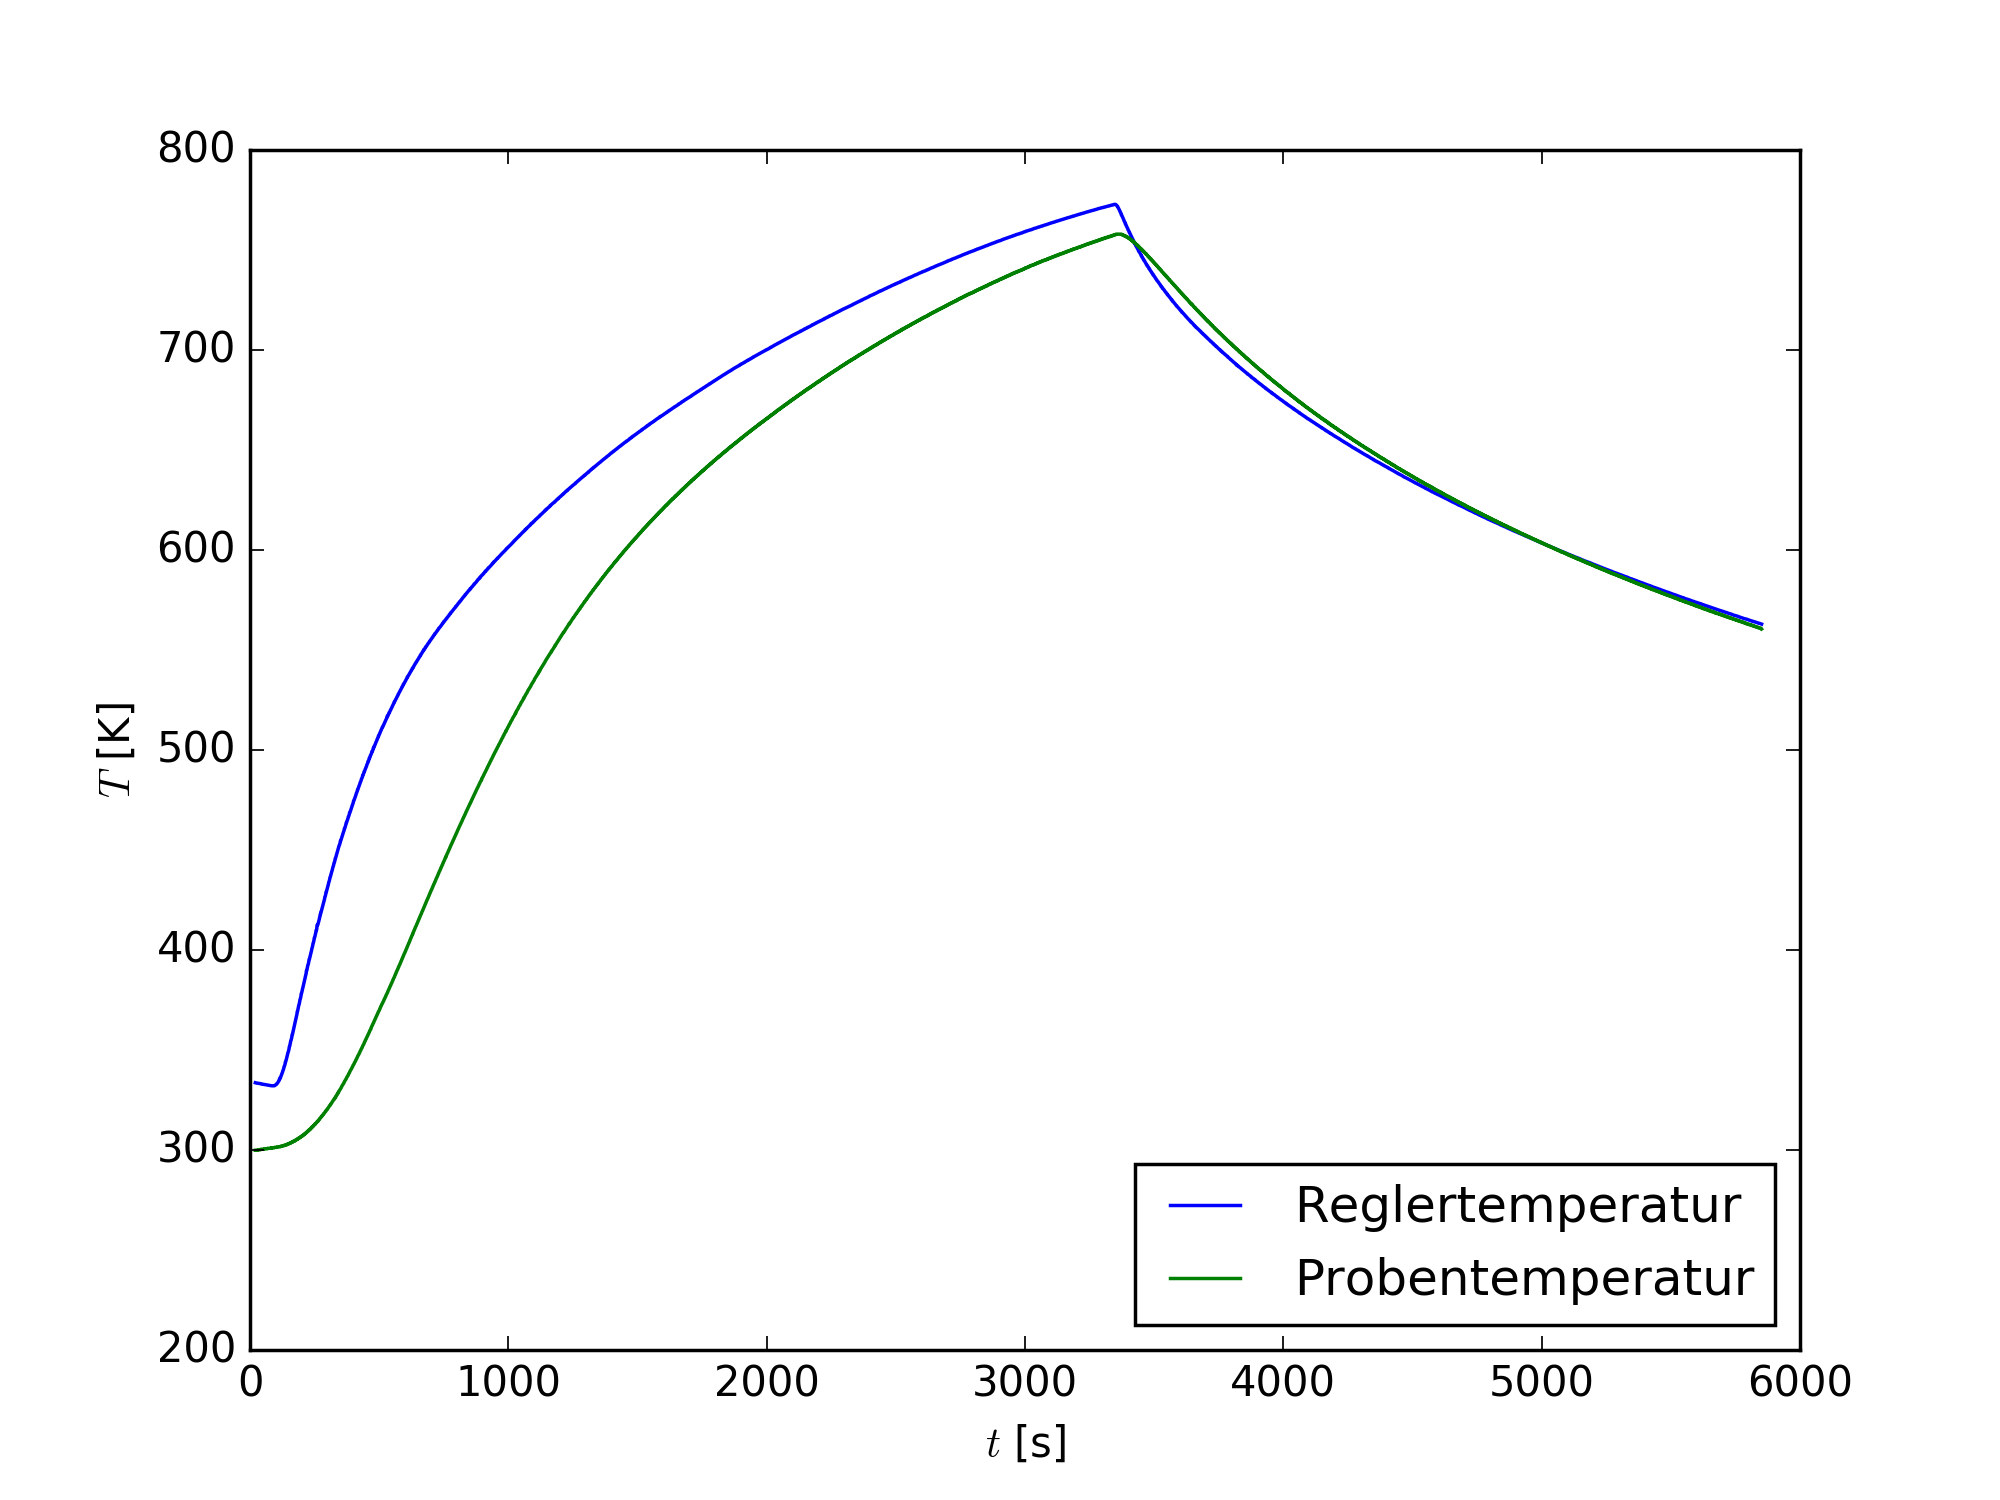
\includegraphics[width=0.9\textwidth]{temp_time.png}
\caption{Temperaturverlauf über die Zeit}
\label{temp_time}
\end{figure}
%

\section{Temperaturabhängigkeit des elektrischen Widerstands}
Die Siliziumprobe wurde zuerst auf $500^{\circ}$C erwärmt und dann wieder auf Raumtemperatur abgekühlt. Während des ganzen Prozesses wurde der elektrische Widerstand mithilfe der Vierpunkt-Messmethode ermittelt. In der Abbildung \ref{res_temp} ist ersichtlich, dass der Widerstandsverlauf bei Aufwärm- (blau) und Abkühlprozess (grün) leicht unterschiedlich ausfällt.
%
\begin{figure}[htbp]
\centering
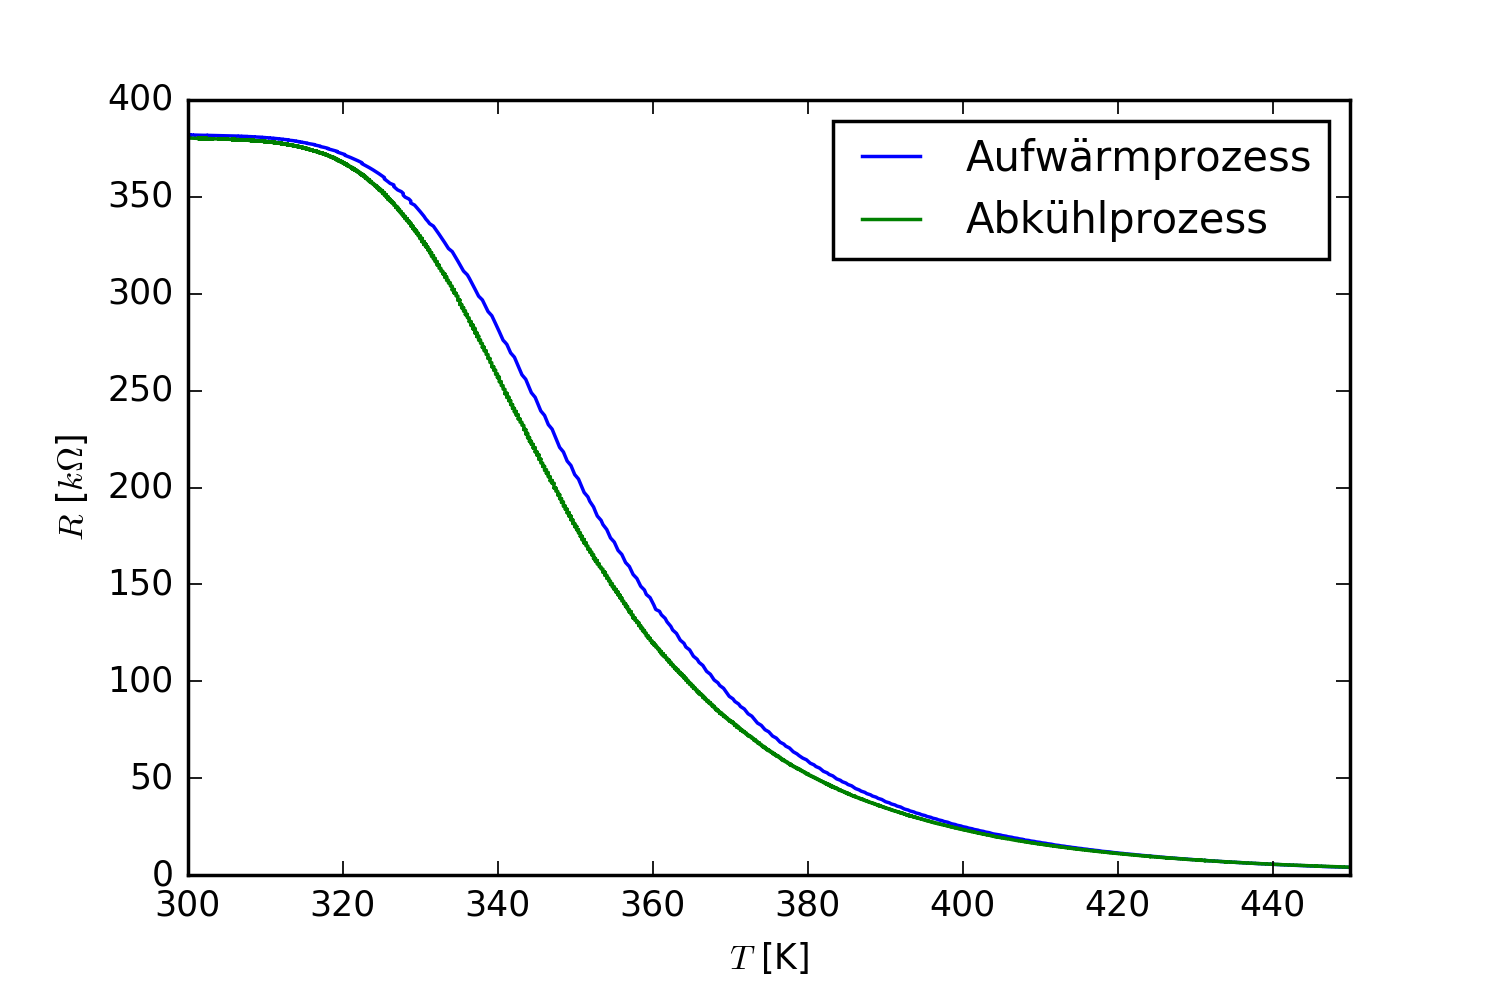
\includegraphics[width=0.9\textwidth]{res_temp.png}
\caption{elektrischer Widerstand des Halbleiters}
\label{res_temp}
\end{figure}
%


\chapter{Auswertung}

Formel \ref{eq:Endloesung} in Kapitel \ref{ch:Physik} vereinfacht sich für T hinreichend klein zu:
\begin{equation}
\label{eq:Rexp}
R \approx B \exp \left(\frac{E_g}{2 k_B T}\right)
\end{equation}
mit einer thermostatischen Proportionalitätskonstante $B$, da die Temperaturabhängigkeit der Exponentialfunktion sehr gross gegenüber dem Beitrag von $T^{-3/2}$ und den Mobilitäten $\mu_e$ und $\mu_h$ ist.
\\
Der Logarithmus der Gleichung \ref{eq:Rexp} ist dann:
\begin{equation}
\label{eq:Rlog}
\ln(R) = \ln (B) + \frac{E_g}{2 k_B} T^{-1}
\end{equation}

Aufgrund der linearen Abhängigkeit von $T^{-1}$ ist es sinnvoll, die Messwerte in einem Plot mit $T^{-1}$ in der x-Achse und ln$(R)$ in der y-Achse darzustellen. Der dadurch entstandene Graph ist grösstenteils näherungsweise linear. Bei kleinen Temperaturen bzeziehungsweise grossem $T^{-1}$ scheitert die Näherung, die in Formel \ref{eq:Rexp} gemacht wurde. Die Steigung $a$ eines linearen Fits durch den näherungsweise linearen Bereich hängt aufgrund von Gleichung \ref{eq:Rlog} direkt mit der Bandlücke zusammen:
\begin{equation}
\label{eq:bandgap}
a = \frac{E_g}{2 k_B} \quad \Rightarrow \quad E_g = 2 k_B a
\end{equation}

Dies wurde einmal für die Messung während des Aufheizens der Probe und einmal für die Messung während des Abkühlens durchgeführt:
\\
\begin{figure}[H]
\centering
    \subfigure{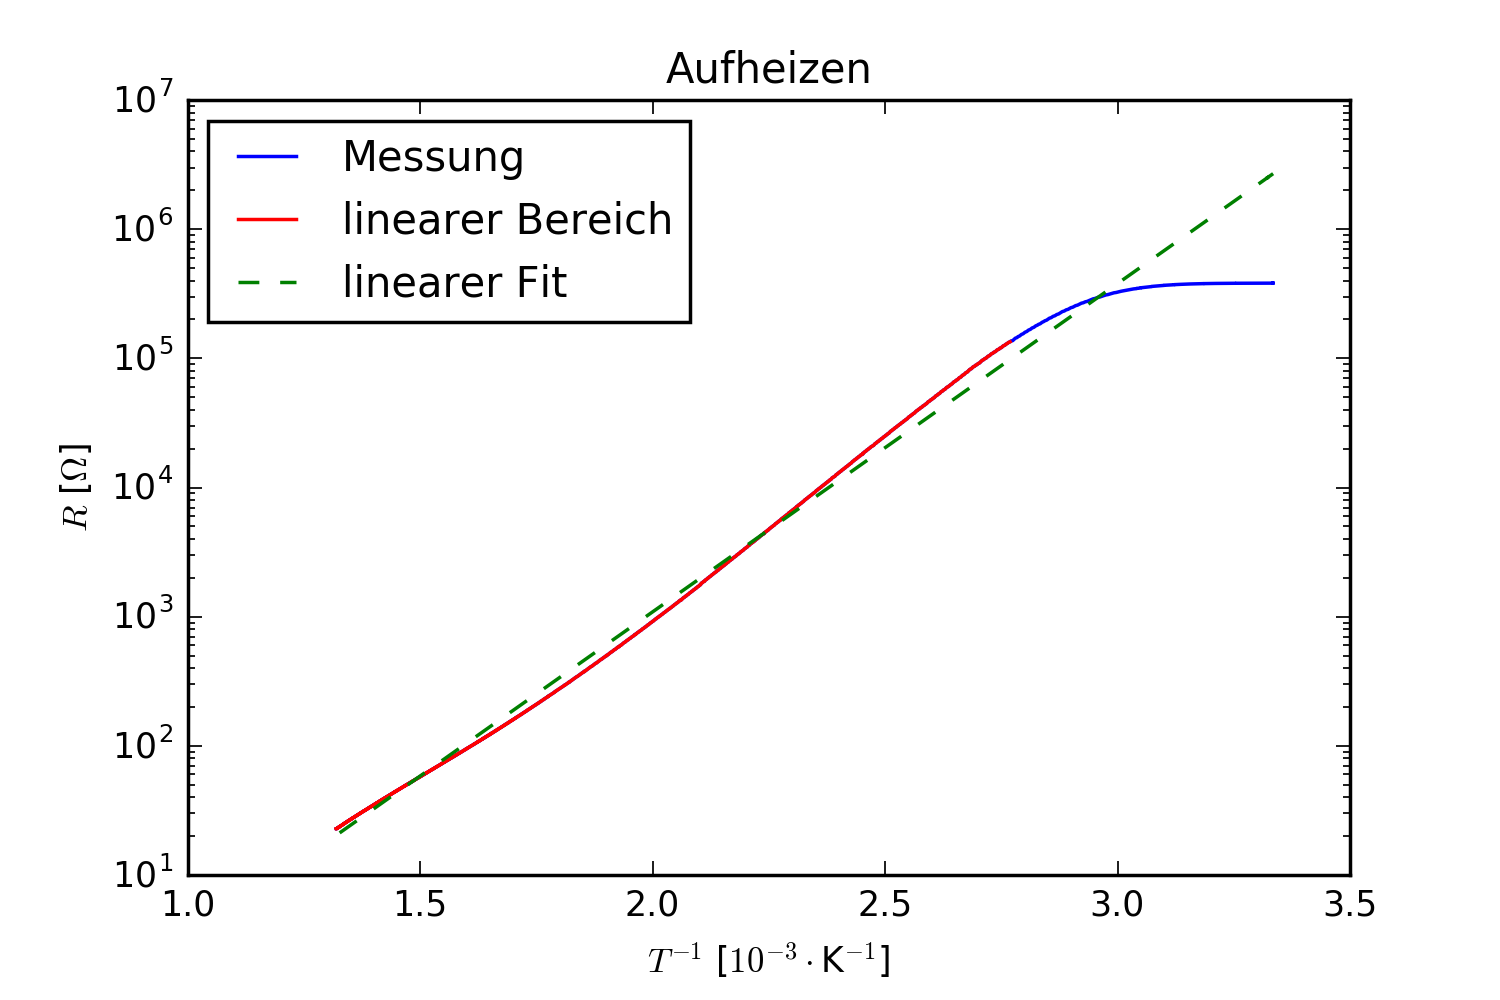
\includegraphics[width=0.45\textwidth]{temp_heat.png}}
    \subfigure{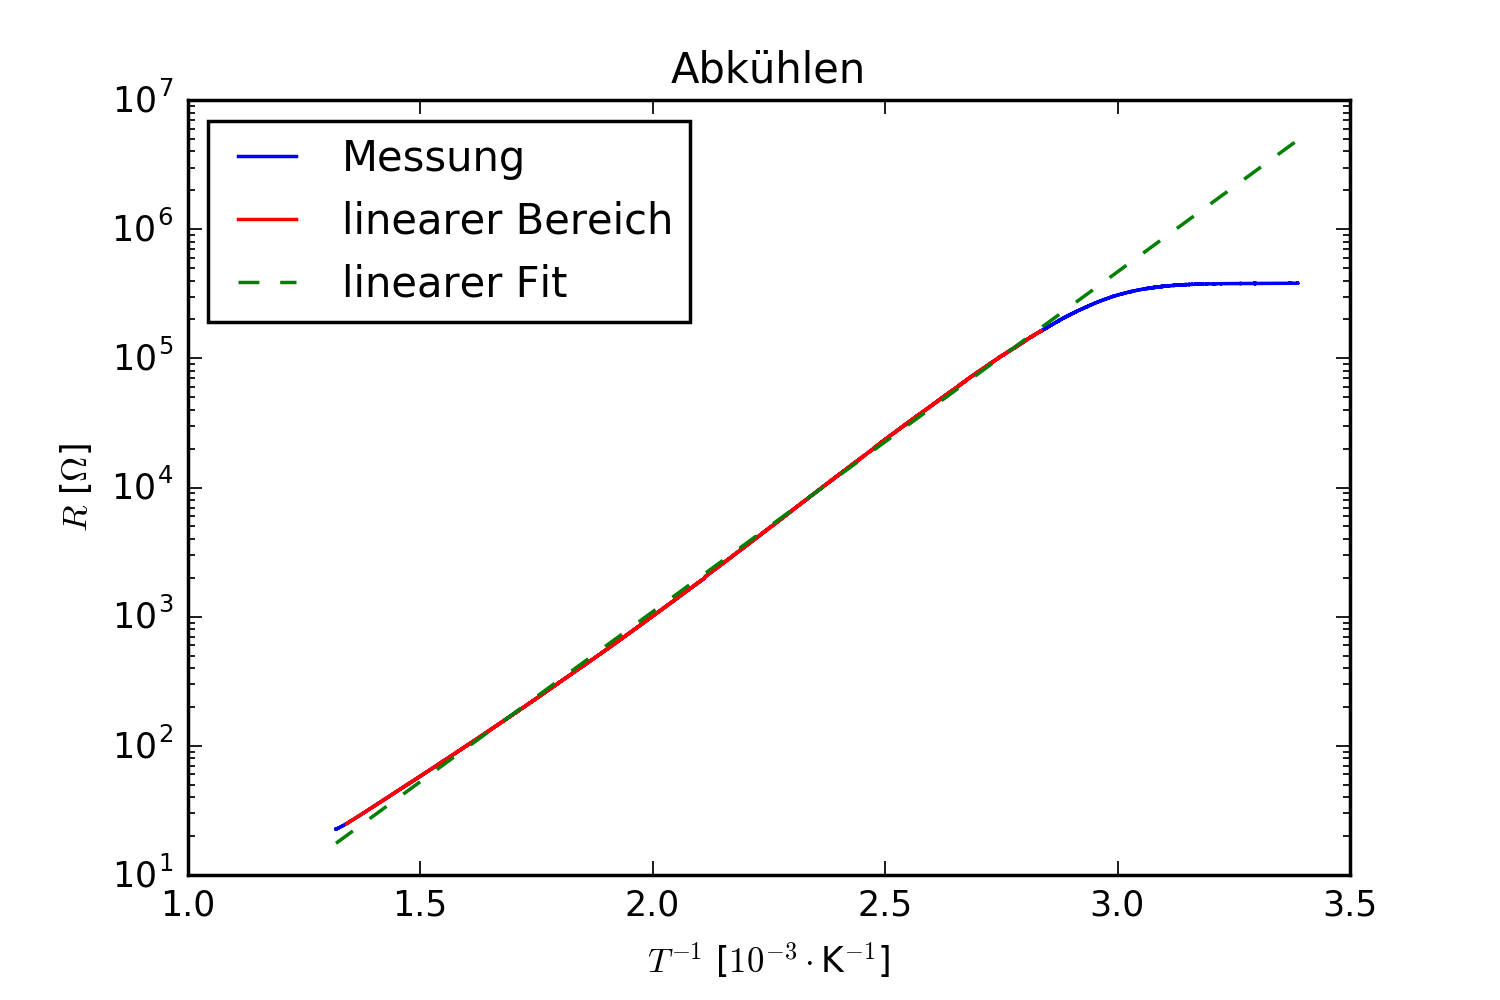
\includegraphics[width=0.45\textwidth]{temp_cool.png}}
\caption{Linearer Fit durch den näherungsweise linearen Bereich der ln$R$($T^{-1}$)-Kurve für die Messung während des Aufheizens links und Abkühlens rechts}
\end{figure}

Der rot eingefärbte Bereich der Messkurve steht für denjenigen Bereich, den wir als näherungsweise linear angenommen haben. Der lineare Fit in der Messung während des Aufheizens hat eine Steigung von $a_1$ = (5854$\pm$7)K und einen y-Achsenabschnitt von $b_1$ = -4.716$\pm$0.012. Beim Abkühlen beträgt die Steigung  $a_2$ = (6061$\pm$1)K und der y-Achsenabschnitt $b_2$ = -5.130$\pm$0.003.
\\
Erstere Messung führt sodann nach Formel \ref{eq:bandgap} zu einer Bandlücke von $E_{g,1}$ = (1.0089$\pm$0.0012)eV und letztere zu $E_{g,2}$ = (1.0446$\pm$0.0002)eV. Hier muss berücksichtigt werden, dass die angegebene Unsicherheit direkt aus dem linearen Fit kommt und


\chapter{Appendix}
\section{Spannungstabelle Thermoelement}
\label{Kacktabelle}
\begin{figure}[htbp]
\centering
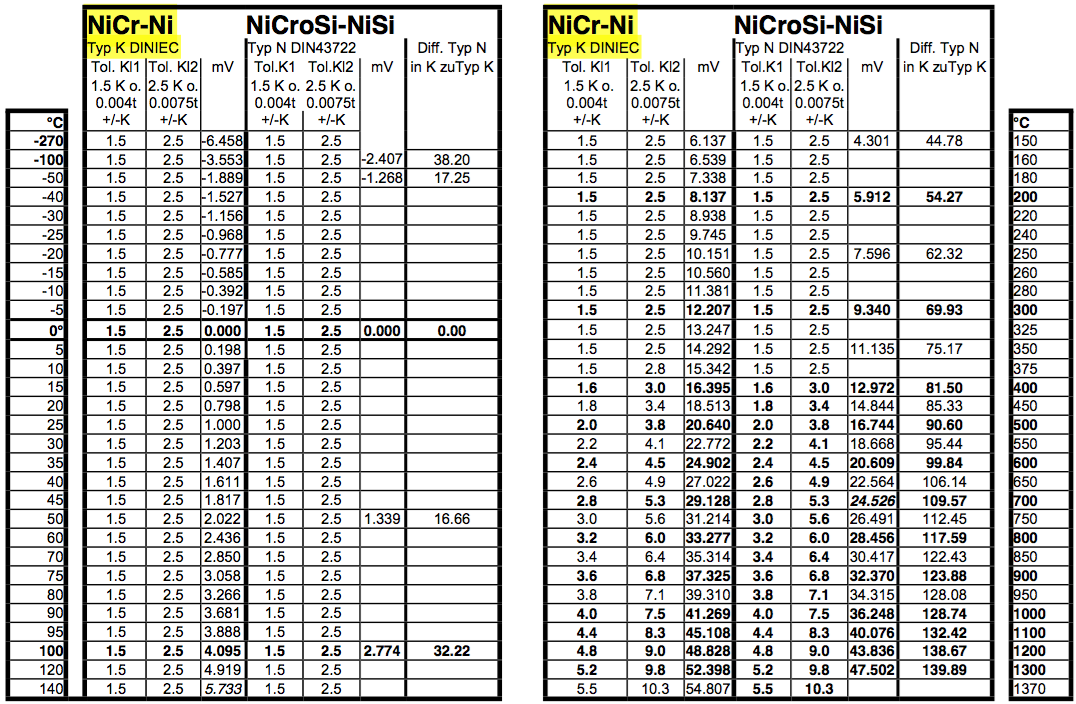
\includegraphics[width=1\textwidth]{spannungstabelle.png}
\label{temp_cool}
\end{figure}
%
Als Bezugspunkt wird in dieser Tabelle die Vergleichsstellentemperatur $T_{0}=0^{\circ}C$ verwendet. Für die Messung bei Raumtemperatur $T_{R} \approx 26^{\circ}C$ muss dies entsprechend kompensiert werden:
$$ U_{th} = U_{1} \, (1-\frac{T_{0}}{T_{R}}) $$


 
 
 
 

%\renewcommand{\bibname}{Quellenverzeichnis}
%\printbibliography

\end{document}
